\documentclass[11pt,a4paper]{article}

\usepackage[utf8]{inputenc}
\usepackage[T1]{fontenc}
\usepackage[english]{babel}
\usepackage{lmodern}
\usepackage[margin=2.5cm]{geometry}
\usepackage{graphicx}
\usepackage{booktabs}
\usepackage{tabularx}
\usepackage{enumitem}
\usepackage[hidelinks]{hyperref}

\setlist{nosep}

\title{Cerio\\[0.3em]\large Project Documentation}
\author{}
\date{\today}

\begin{document}

\maketitle
\tableofcontents
\newpage

% ------------------------------------------------------------
\section{Overview}

The subject of the project is the development of a two-dimensional platform game in the style
of Mario or Celeste (reference subject to change) and, as its main part, the design of
algorithms and models for automatic level completion by a bot.

% ------------------------------------------------------------
\section{Game rules}

The main goal of the game is to reach the exit. The game consists of procedurally generated
levels. Death sends the player back to the start of the level. Each level contains:
\begin{itemize}
  \item a level entrance and exit,
  \item an area in which the player can move,
  \item stationary obstacles capable of killing the player.
\end{itemize}
Some levels also contain interactive elements, e.g.\ buttons. Completing a level activates
a checkpoint, so it does not have to be repeated.

\subsection{Game goals}

\begin{description}
  \item[Main goal:] reaching the level exit.
  \item[Intermediate goals:] avoiding obstacles, activating interactive elements,
        managing stamina, reaching checkpoints.
  \item[Bonus goals:] collecting bonus points (coins).
  \item[Failure condition:] contact with an obstacle, which restarts the level.
\end{description}

\subsection{Game mechanics}

\begin{itemize}
  \item wall climbing,
  \item traversing dynamic levels,
  \item avoiding obstacles,
  \item stamina mechanics,
  \item interaction with the environment (buttons, levers),
  \item elements that kill the character,
  \item bonus points (coins) and other collectibles.
\end{itemize}

\textbf{Available movement actions:} dash, move left, move right, jump, crouch, climb.

% ------------------------------------------------------------
\section{Bot}

\subsection{Operation}

The bot runs inside the game, without the graphics layer. Instead of an image, it reads game
metadata: the level layout, obstacles, interactive elements and the character state
(position, velocity, stamina).

Based on this data, it selects successive actions and moves towards the exit. Decisions are
made either by an algorithm searching the space of possible moves or by a trained model.

The bot completes previously unseen procedural levels.

\subsection{Planner}

The planner is a state-space search algorithm (A*) that, before moving, computes a sequence
of actions leading to the exit. For the current game state it simulates the effects of the
available actions, discards moves that end in death or lead to already visited states, and
expands the states closest to the exit first. Deterministic game physics is a necessary
condition.

The planner serves three purposes:
\begin{enumerate}
  \item it is the v1 bot (algorithmic approach),
  \item it verifies that procedurally generated levels can be completed,
  \item it provides demonstrations for training the v2 model (PyTorch).
\end{enumerate}

% ------------------------------------------------------------
\section{Requirements}

\subsection{Performance requirements}

Minimum hardware configuration: AMD Ryzen 5 7600X (6 cores), NVIDIA GeForce RTX 3070,
48~GB RAM. Resolution $854\times480$~px, maintained for 80\% of the gameplay, assuming the
game is ``playable''.

\subsection{Evaluation criteria}

\begin{itemize}
  \item The bot must complete at least 70\% of a test set consisting of 10 levels.
  \item The bot must complete the task in finite time, shorter than three times the
        human completion time.
\end{itemize}

\subsection{Technology stack}

Python, Pygame, PyTorch.

% ------------------------------------------------------------
\section{Schedule}

\begin{table}[h]
\centering
\begin{tabularx}{\textwidth}{@{}l l X@{}}
\toprule
\textbf{Date} & \textbf{Checkpoint} & \textbf{Scope} \\
\midrule
08.10.2026 & Project requirements & Requirements, game goals, bot assumptions \\
22.10.2026 & Report & Game engine basics, deterministic physics, level format \\
05.11.2026 & Milestone I & Full game mechanics, environment interface, bot v1 (planner) \\
19.11.2026 & Report & Procedural generator, human time measurement, test set \\
03.12.2026 & Deadline & Bot v2, evaluation, optimization, final report \\
\bottomrule
\end{tabularx}
\caption{Project checkpoints}
\end{table}

\begin{figure}[h]
\centering
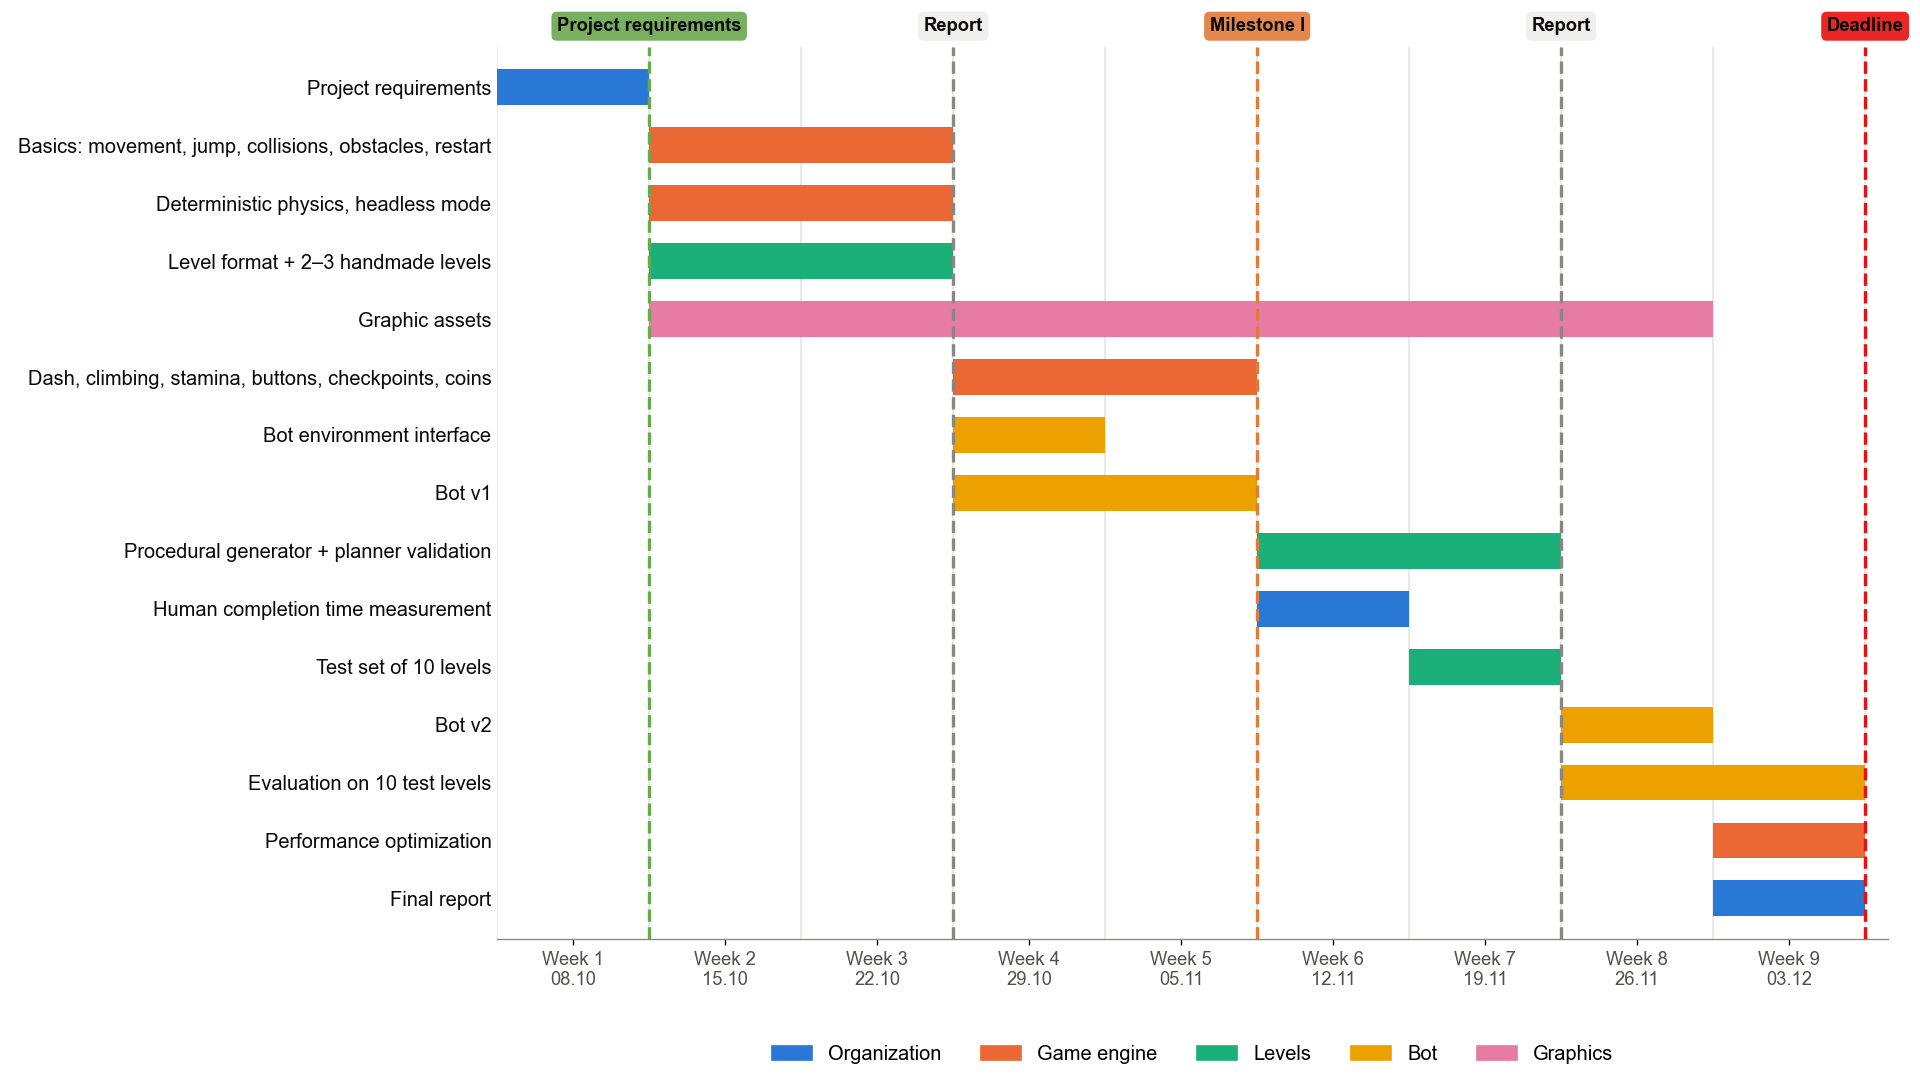
\includegraphics[width=\textwidth]{gantt-chart.png}
\caption{Gantt chart}
\end{figure}

\end{document}
